% ch9.tex
% This work is licensed under the Creative Commons Attribution-Noncommercial-Share Alike 3.0 New Zealand License.
% To view a copy of this license, visit http://creativecommons.org/licenses/by-nc-sa/3.0/nz
% or send a letter to Creative Commons, 171 Second Street, Suite 300, San Francisco, California, 94105, USA.


\chapter{Um pouco sobre gráficos}\label{ch:abitgraphic}

O problema de usar a tartaruga para desenhar, é$\ldots$ que$\ldots$$\ldots$ as tartarugas$\ldots$$\ldots$$\ldots$ são$\ldots$$\ldots$$\ldots$$\ldots$muito$\ldots$$\ldots$$\ldots$$\ldots$ lentas.
\par
Mesmo quando uma tartaruga está no seu máximo de velocidade, ela ainda não está indo rápido. Para tartarugas, isso não é um problema --- eles tem tempo a perder ---- mas quando estamos falando de gráficos de computador, isso é um problema. Se você tem um Nintendo DS, um Gameboy Advance ou jogos no seu computador, pense por um momento sobre os gráficos (que você vê na tela). Existem diversas formas de exibição de gráficos que são usadas em jogos: existem os jogos 2d (ou de 2 dimensões), onde as imagens são planas e os personagens geralmente se movem para cima, para baixo, esquerda e direita --- muitoc omum em videogames de mão --- e finalmente, os jogos 3d, onde as figuras desenhadas na tela tentando imitar a realidade.

Todos estes tipos de gráficos tem uma coisa em comum --- eles precisam ser desenhados muito rapidamente. Você já tentou fazer a sua própria animação? Onde você pega um bloco de folhas de papel e no canto, na parte debaixo da primeira página, e na próxima folha, você desenha a figura um pouco mais para frente e por assim em diante. Quando você terminar, você folheia as páginas e se você folhear rápido o suficiente, vai parecer que a figura está realmente se movendo. É assim que basicamente todas as animações são feitas --- se forem os desenhos que você assiste na tv ou os jogos que você joga no videogame ou computador. Você desenha algo e depois desenha a mesma coisa novamente, com pequenas mudanças, para dar a ilusão de movimento. Que é o motivo pelo qual a tartaruga não é tão boa fazendo gráficos. Para fazer uma imagem parecer que está se movendo, você precisa desenhar cada `frame' (quadro) da animação muito rapidamente.
\par
Gráficos tridimensionais são feitos de uma maneira bem diferente dos gráficos bidimensionais, mas ainda assim, a ideia básica é a mesma. No momento em que a sua tartaruga terminou de desenhar uma pequena porção de uma figura, já seria hora de virar a página e começar a desenhar a próxima$\ldots$

\begin{center}
\includegraphics*[width=100mm]{eps/turtle1.eps}
\end{center}

\section{Desenhar rapidamente}

Cada linguagem de programação tem um método diferente de desenhar na tela. Alguns métodos são mais rápidos, enquanto outros são mais lentos, o que significa que os programadores que criam jogos tem que ser cuidadosos na hora de escolher a linguagem que vão usar para trabalhar.
\par
Assim como o Python também possui diversas formas diferentes de fazer gráficos (incluindo a tartaruga, que nós já usamos), mas os melhores métodos (do ponto de vista dos gráficos) normalmente são módulos e bibliotecas que são incluidas no Python por padrão. Você provavelmente terá que programar por alguns anos para poder instalar e usar algumas dessas bibliotecas complexas.

Felizmente, existe um módulo que vem com o Python, que podemos usar para fazer gráficos simples (um pouco mais rápido que a tartaruga). Talvez rápida o suficiente para a chamarmos de Tartaruga Rápida para Desenhar.

\begin{center}
\includegraphics*[width=100mm]{eps/turtle2.eps}
\end{center}

O módulo se chama \code{tkinter}\index{modules!tkinter} (um nome estrenho, que vem de `Tk interface') e pode ser usada para criar aplicações completas (você pode até mesmo criar um Editor de Textos se quiser), assim como apenas desenhar. Nós podemos criar uma aplicação simples com um botão, usando o seguinte código:

\begin{listing}
\begin{verbatim}
1. >>> from tkinter import Tk, Button
2. >>> tk = Tk()
3. >>> btn = Button(tk, text="clique aqui")
4. >>> btn.pack()
\end{verbatim}
\end{listing}

Na linha 1, nós importamos o que vamos usar do módulo \code{Tk} --- o mais usado é o \code{Tk}, que cria uma janela básica que podemos adicionar algumas coisas. Ela aparecerá na tela assim que você digitar a linha 2. Na linha 3, nós criamos um novo botão (`Button') e o associamos à variável \code{btn}. O botão é criado passando o objeto \code{tk} como parâmetro, junto de um parâmetro nomeado com as palavras `clique aqui'.

\par
\fbox{\colorbox{PaleBlue}{\parbox{.75\linewidth} {
\section*{Parâmetros Nomeados}

Essa é a primeira vez que nós usamos os `parâmetros nomeados'\index{named parameters}. Eles funcionam da mesma forma que os parâmetros normais, exceto que eles podem aparecer em qualquer ordem, então nós devemos nomeá-los.

Por exemplo, suponha que nós tivessemos uma função `retangulo' que recebe dois parâmetros: largura e altura. Normalmente, nós deveríamos chamar essa função usando algo do tipo \code{retangulo(200, 100)}, que significa que nós queremos um retangulo de 200 pixels de largura, por 100 de altura. Mas e se os parâmetros pudessem aparecer em qualquer ordem? Como saberíamos qual é a largura e qual é a altura?

Nesse caso, seria melhor dizer exatamente o que é o que. Por exemplo: \code{retangulo(altura=100, largura=200)}. Na realidade, a ideia dos parâmetros nomeados é um pouco mais complicada do que isso e pode ser usada de diversas maneiras, para tornar as funções mais flexíveis --- mas isso é assunto para um livro mais aprofundado do que essa introdução à programação.
\par
}}}
\par

A última linha (4) é uma instrução que diz ao botão para se desenhar. Nesse ponto, a janela criada na linha 2 irá encolher para o tamanho de um pequeno botão, contendo as palavras `clique aqui'. Algo parecido com isso:

\begin{center}
\includegraphics*[width=30mm]{eps/figure31.eps}
\end{center}

O botão não faz nada demais, mas você pode ao menos clicar nele. Nós podemos fazer com que ele faça algo, modificando um pouco o exemplo anterior (assegure que a janela que criamos anteriormente está fechada). Primeiro, nós criamos uma função que imprime um texto:

\begin{listing}
\begin{verbatim}
>>> def ola():
...     print('ola!')
\end{verbatim}
\end{listing}

\noindent
Então, modificamos o nosso exemplo para usar a função:

\begin{listing}
\begin{verbatim}
>>> from tkinter import *
>>> tk = Tk()
>>> btn = Button(tk, text="clique aqui", command=ola)
>>> btn.pack()
\end{verbatim}
\end{listing}

O parâmetro nomeado `command' diz que nós queremos acionar a função \code{ola}, quando o botão for clicado. Logo, se você clicar no botão, você verá a mensagem ``ola!'' no terminal --- impressa cada vez que você clicar no botão.

\section{Desenhando algo simples}

Botões não ajudam muito quando o que você quer é desenhar algo na tela --- então nós precisamos usar um componente diferente: um \code{Canvas}\index{modules!tkinter!Canvas} (tela). Quando criamos um `canvas', diferente do botão (que recebe os parâmetros `texto' e `comando'), nós precisamos passar a largura e a altura (em pixels), da tela. Tirando isso, o código é similar ao do botão:

\begin{listing}
\begin{verbatim}
>>> from tkinter import *
>>> tk = Tk()
>>> canvas = Canvas(tk, width=500, height=500)
>>> canvas.pack()
\end{verbatim}
\end{listing}

Similar ao exemplo do botão, uma janela aparecerá quando você digitar a linha 2. E na linha 4, a janela aumentará seu tamanho. Nós podemos desenhar uma linha na tela, usando pixels como coordenadas. Coordenadas são as posições dos pixels em uma tela. Na tela (ou `canvas') do Tk, as coordenadas dizem qual a largura (da esquerda para a direita) e a altura (do topo até embaixo). A parte do `da esquerda para a direita' é chamada de eixo-x, enquanto o `do topo até embaixo' é chamado de eixo-y.

\begin{figure}
\begin{center}
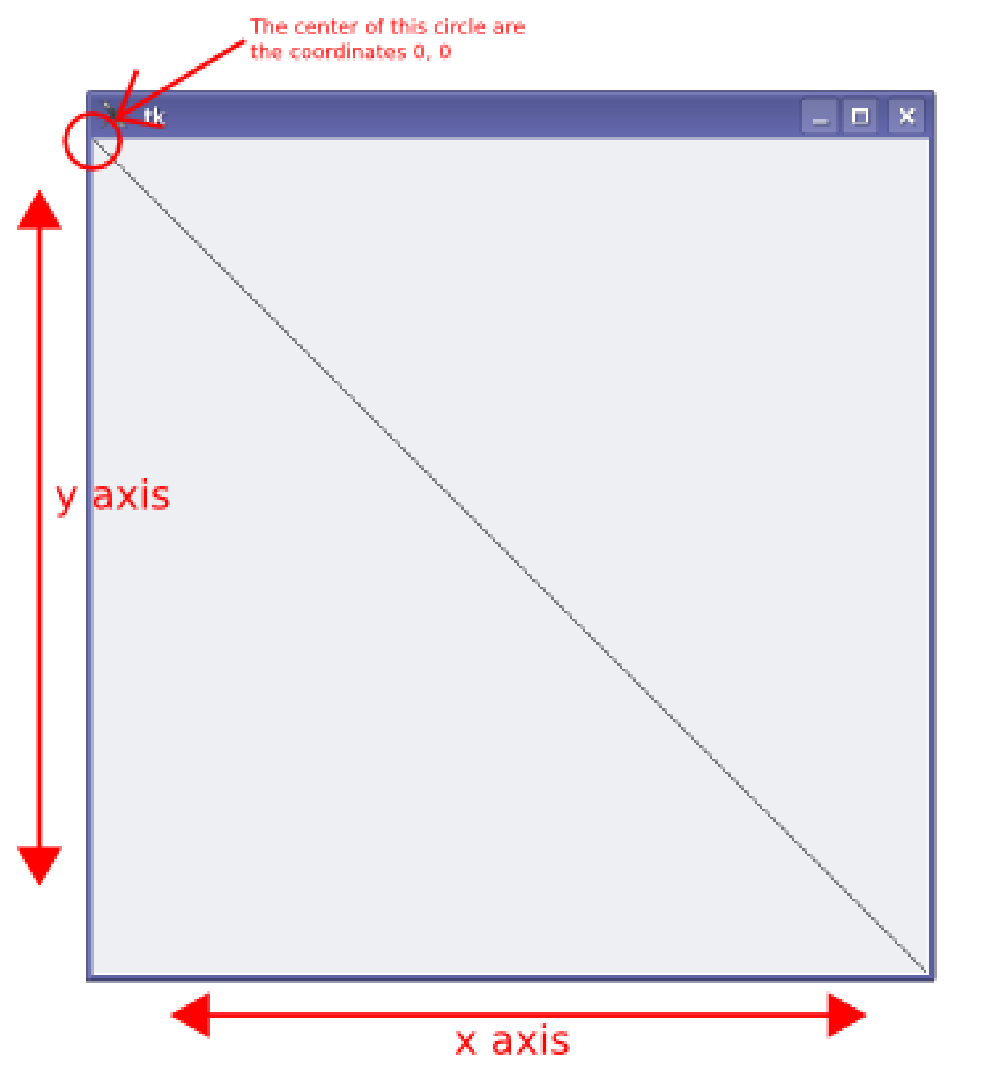
\includegraphics[width=80mm]{eps/figure32.eps}
\end{center}
\caption{Eixo-x e eixo-y da tela.}\label{fig32}
\end{figure}

Como a tela tem 500 pixels de largura e 500 de altura, as coordenadas do canto inferior direito da tela são 500, 500. Então, a linha na figura~\ref{fig32} pode ser desenhada iniciando das coordenadas 0, 0 e terminadas nas coordenadas 500, 500.\index{modules!tkinter!create\_line}:

\begin{listing}
\begin{verbatim}
>>> from tkinter import *
>>> tk = Tk()
>>> canvas = Canvas(tk, width=500, height=500)
>>> canvas.pack()
>>> canvas.create_line(0, 0, 500, 500)
\end{verbatim}
\end{listing}

\noindent
Agora, para fazer a mesma coisa com a tartaruga, precisariamos usar o seguinte código:

\begin{listing}
\begin{verbatim}
>>> import turtle
>>> turtle.setup(width=500, height=500)
>>> t = turtle.Pen()
>>> t.up()
>>> t.goto(-250, 250)
>>> t.down()
>>> t.goto(500, -500)
\end{verbatim}
\end{listing}

Assim vemos que o código usando o \code{tkinter} já é uma melhoria, menor e menos complicado. Existe um grande número de métodos disponíveis no objeto Canvas, alguns que não nos serão tão úteis, mas veremos alguns exemplos interessantes.

\section{Desenhando Caixas}

Com a tartaruga, nós desenhamos uma caixa movendo para frente, virando, para frente, virando novamente e por assim em diante. Eventualmente você pode desenhar um retângulo ou um quadrado apenas mudando o quanto ``para frente'' você quer mover. Com o tkinter, desenhar um quadrado ou um retângulo é bem mais simples --- você apenas precisa saber as coordenadas dos cantos.

\begin{listingignore}
\begin{verbatim}
>>> from tkinter import *
>>> tk = Tk()
>>> canvas = Canvas(tk, width=400, height=400)
>>> canvas.pack()
>>> canvas.create_rectangle(10, 10, 50, 50)
1
\end{verbatim}
\end{listingignore}

No exemplo acima, nós criamos uma tela com 400 pixels de largura, 400 pixels de altura e então nós desenhamos um quadrado no canto superior esquerdo (10 pixels da esquerda para a direita e 10 pixels do topo para baixo). Você deve estar se perguntando: que número é aquele que apareceu após digitar o \code{create\_rectangle}\index{modules!tkinter!create\_rectangle}? Isso é um número de identificação para a forma que nós desenhamos (seja uma linha, um quadrado ou um círculo). Nós falaremos desse número mais tarde.

Portanto, os parâmetros passados para o \code{create\_rectangle} são: posição do canto superior esquerdo, posição do canto inferior esquerdo, posição do canto superior direito e posição do canto inferior direito. Para não termos que digitar tudo isso toda vez, vamos nos referir à essas posições como x1, y2 e x2, y2. Nós podemos desenhar um retângulo apenas usando um número maior no x2:

\begin{listing}
\begin{verbatim}
>>> canvas.create_rectangle(100, 100, 300, 50)
\end{verbatim}
\end{listing}

\noindent
Ou usando um número maior no y2:

\begin{listing}
\begin{verbatim}
>>> canvas.create_rectangle(100, 200, 150, 350)
\end{verbatim}
\end{listing}

O último retângulo está basicamente dizendo: vá 100 pixels pela tela (a partir do canto superior esquerdo), 200 pixels para baixo e então desenhe uma caixa, saindo do pixel 150 até o 350. Nesse momento, você terá algo como a figura~\ref{fig33} na sua tela.

\begin{figure}
\begin{center}
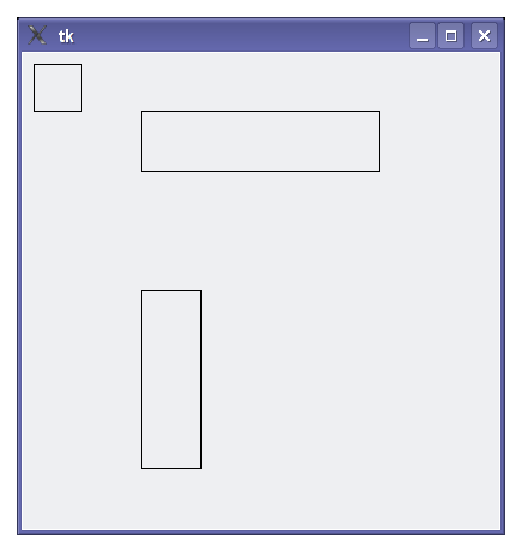
\includegraphics[width=80mm]{eps/figure33.eps}
\end{center}
\caption{caixas no tkinter.}\label{fig33}
\end{figure}

Vamos tentar preencher o canvas com retângulos de diferentes tamanhos. Nós podemos fazer isso usando o módulo \code{random}\index{modules!random}. Primeiro, importe o módulo `random':

\begin{listing}
\begin{verbatim}
>>> import random
\end{verbatim}
\end{listing}

Então em seguida, nós podemos criar uma função que usa um número aleatório para as coordenadas do canto superior e inferior. A função que vamos usar chama \code{randrange}\index{modules!random!randrange}:

\begin{listing}
\begin{verbatim}
>>> def retangulo_aleatorio(largura, altura):
...     x1 = random.randrange(largura)
...     y1 = random.randrange(altura)
...     x2 = random.randrange(x1 + random.randrange(largura))
...     y2 = random.randrange(y1 + random.randrange(altura))
...     canvas.create_rectangle(x1, y1, x2, y2)
\end{verbatim}
\end{listing}

Nas primeiras duas linhas, nós definimos as variáveis com as coordenadas dos cantos superior e inferior esquerdo do retângulo, usando o \code{randrange}, passando a largura e a altura. A função \code{randrange}, recebe um número como argumento (veja o Apêndice~\ref{app:afewpythonmodules} para mais detalhes do \code{randrange}) --- então \code{randrange(10)} retorna um número entre 0 e 9, \code{randrange(100)}, retorna um número entre 0 e 99 e por assim em diante. As próximas duas linhas, definem variáveis com as coordenadas dos cantos superior e inferior direito do retângulo (ou quadrado!) --- nós usamos as coordenadas do canto superior e inferior esquerdo (x1 e y1) para somar à um número aleatório nas variáveis e finalmente chamamos a função \code{create\_rectangle} usando essas variáveis. Você pode tentar usar a função \code{retangulo\_aleatorio}, passando a largura e a altura da tela (canvas) que você criou:

\begin{listing}
\begin{verbatim}
>>> retangulo_aleatorio(400, 400)
\end{verbatim}
\end{listing}

\noindent
Ou, para preencher a tela, que tal fazermos um laço para chamar essa função várias vezes:

\begin{listing}
\begin{verbatim}
>>> for x in range(0, 100):
...     retangulo_aleatorio(400, 400)
\end{verbatim}
\end{listing}

\noindent
Que faz um pouco de bagunça (figura~\ref{fig34}, mas que é interessante.

\begin{figure}
\begin{center}
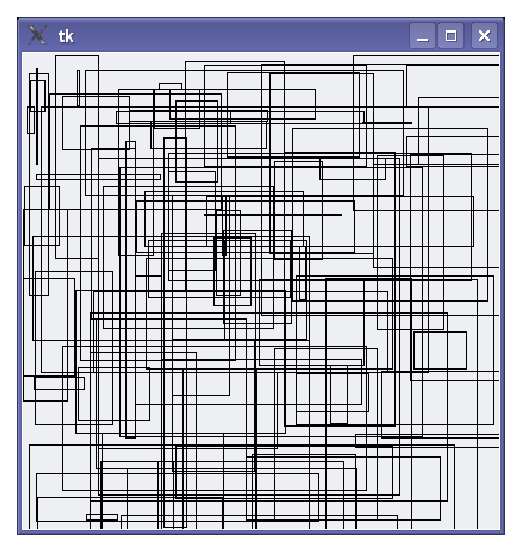
\includegraphics[width=80mm]{eps/figure34.eps}
\end{center}
\caption{Uma bagunça de retângulos.}\label{fig34}
\end{figure}

Lembra-se no último capítulo, que nós definimos cores para a tartaruga desenhar, usando as porcentagens de 3 cores: vermelho, verde e azul? Com o \code{tkinter} você pode fazer o mesmo, mas infelizmente, é um pouco mais complicado que o módulo \code{turtle}. Primeiramente, vamos alterar a função \code{retangulo\_aleatorio} para aceitar uma cor de preenchimento como parâmetro:

\begin{listing}
\begin{verbatim}
>>> def retangulo_aleatorio(largura, altura, cor_preencher):
...     x1 = random.randrange(largura)
...     y1 = random.randrange(altura)
...     x2 = random.randrange(x1 + random.randrange(largura))
...     y2 = random.randrange(y1 + random.randrange(altura))
...     canvas.create_rectangle(x1, y1, x2, y2, fill=preencher_cor)
\end{verbatim}
\end{listing}

A função \code{create\_rectangle} da tela, pode receber um parâmetro `fill' que define uma cor para preenchimento. Nós podemos passá-la pela função. Tente o seguinte:

\begin{listing}
\begin{verbatim}
>>> retangulo_aleatorio(400, 400, 'green')
>>> retangulo_aleatorio(400, 400, 'red')
>>> retangulo_aleatorio(400, 400, 'blue')
>>> retangulo_aleatorio(400, 400, 'orange')
>>> retangulo_aleatorio(400, 400, 'yellow')
>>> retangulo_aleatorio(400, 400, 'pink')
>>> retangulo_aleatorio(400, 400, 'purple')
>>> retangulo_aleatorio(400, 400, 'violet')
>>> retangulo_aleatorio(400, 400, 'magenta')
>>> retangulo_aleatorio(400, 400, 'cyan')
\end{verbatim}
\end{listing}

Alguns, talvez todas, as cores funcionarão pelo nome. Mas algumas delas irão resultar uma mensagem de erro (depende se você estiver no Windows, no Mac ou no Linux). Bem fácil até agora. E se nós quisermos uma cor ouro? No módulo \code{turtle}, nós criamos a cor ouro usando 100\% do vermelho, 85\% do verde e nada de azul. No \code{tkinter}, nós podemos fazer a cor ouro usando:

\begin{listing}
\begin{verbatim}
>>> retangulo_aleatorio(400, 400, '#ffd800')
\end{verbatim}
\end{listing}

Que, apesar de tudo, é uma forma bem estranha de criar uma cor. `ffd800' é o que chamamos de hexadecimal\index{hexadecimal colors}, e é outra maneira de representar números. Explicar como funcionam os números hexadecimais nos levaria a escrever mais algumas páginas, então para economizá-las, vamos usar a seguinte função para criar cores em hexadecimal:

\begin{listing}
\begin{verbatim}
>>> def corhex(vermelho, verde, azul):
...     vermelho = 255 * (vermelho / 100.0)
...     verde = 255 * (verde / 100.0)
...     azul = 255 * (azul / 100.0)
...     return '#%02x%02x%02x' % (vermelho, verde, azul)
\end{verbatim}
\end{listing}

Chamando `corhex' com 100\% de vermelho, 85\% de verde e 0\% de azul, resultará no código hexadecimal para a cor ouro, que nós queremos:

\begin{listing}
\begin{verbatim}
>>> print(corhex(100, 85, 0))
#ffd800
\end{verbatim}
\end{listing}

\noindent
Você pode criar um rosa choque, usando 98\% de vermelho, 1\% de verde e 77\% de azul:

\begin{listing}
\begin{verbatim}
>>> print(corhex(98, 1, 77))
#f902c4
\end{verbatim}
\end{listing}

\noindent
E você pode usar isso, junto com a função \code{retangulo\_aleatorio} que nós criamos:

\begin{listing}
\begin{verbatim}
>>> retangulo_aleatorio(400, 400, hexcolor(98, 1, 77))
\end{verbatim}
\end{listing}

\begin{figure}
\begin{center}
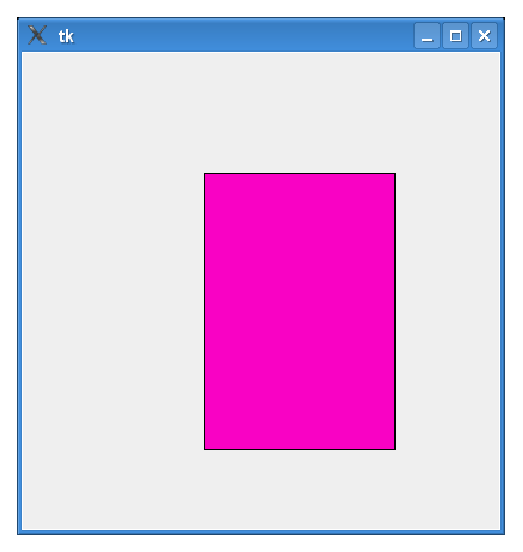
\includegraphics[width=80mm]{eps/figure35.eps}
\end{center}
\caption{Um retângulo rosa.}\label{fig35}
\end{figure}

\section{Desenhando Arcos}

Um arco é uma parte de um círculo, mas para desenhar um com o tkinter, você precisa desenhar um retângulo. Não faz muito sentido, até que você tente desenhar um retangulo e então desenhar um arco dentro dele (veja na figura~\ref{fig36}). O código para desenhar esse arco é mais ou menos assim:

\begin{listing}
\begin{verbatim}
canvas.create_arc(10, 10, 200, 100, extent=180, style=ARC)
\end{verbatim}
\end{listing}

\begin{figure}
\begin{center}
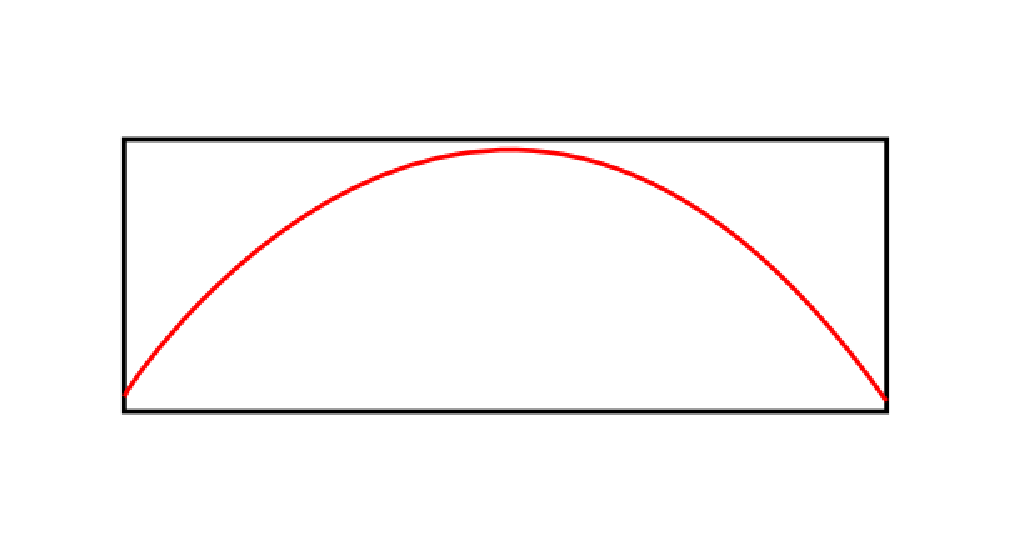
\includegraphics[width=80mm]{eps/figure36.eps}
\end{center}
\caption{Um arco dentro de um retângulo.}\label{fig36}
\end{figure}

Isso posiciona o canto superior esquerdo do retângulo nas coordenadas 10, 10 (10 para o lado e 10 pixels para baixo), e o canto inferior direito do retângulo nas coordenadas 200, 100 (200 pixels para o lado e 100 para baixo). O próximo parâmetro (um parâmetro \textbf{nomeado}), `extent' é usado para especificar os graus do ângulo do arco. Se você não sabe nada sobre graus em um círculo (ou arco), então apenas se lembre que, quando falamos em um círculo, 180 graus formam a metade de um círculo (ou arco), 359 graus formam um círculo completo, 90 graus formam 1/4 de um círculo e 0 graus formam$\ldots$ bem, nada. Aqui está um código que gera um monte de arcos diferentes, então você pode perceber as diferenças básicas quando usamos graus diferentes (você pode ver os exemplos na figura~\ref{fig37}):

\begin{listing}
\begin{verbatim}
>>> canvas.create_arc(10, 10, 200, 80, extent=45, style=ARC)
>>> canvas.create_arc(10, 80, 200, 160, extent=90, style=ARC)
>>> canvas.create_arc(10, 160, 200, 240, extent=135, style=ARC)
>>> canvas.create_arc(10, 240, 200, 320, extent=180, style=ARC)
>>> canvas.create_arc(10, 320, 200, 400, extent=359, style=ARC)
\end{verbatim}
\end{listing}

\begin{figure}
\begin{center}
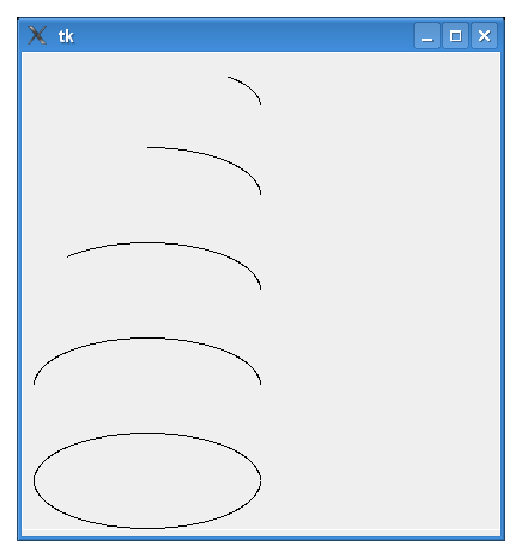
\includegraphics[width=80mm]{eps/figure37.eps}
\end{center}
\caption{Arcos em diferentes graus.}\label{fig37}
\end{figure}

\section{Desenhos Ovais}

Apesar de o último comando acima reproduzir um desenho oval, você também pode usar a função \code{create\_oval}\index{modules!tkinter!create\_oval}. Da mesma maneira que desenhar arcos, uma forma oval é desenhada dentro dos limites de um retângulo. Por exemplo, o seguinte código:

\begin{listing}
\begin{verbatim}
>>> tk = Tk()
>>> canvas = Canvas(tk, width=400,height=400)
>>> canvas.pack()
>>> canvas.create_oval(1, 1, 300, 200)
\end{verbatim}
\end{listing}

Este exemplo desenha uma forma oval dentro do quadrado (imaginário) desenhado nas posições 1, 1 e 300, 200. Se nós desenharmos um retângulo vermelho com as mesmas coordenadas, veremos que a forma oval é desenhada dentro (figura~\ref{fig38}):

\begin{listing}
\begin{verbatim}
>>> canvas.create_rectangle(1, 1, 300, 200, outline="#ff0000")
\end{verbatim}
\end{listing}

\begin{figure}
\begin{center}
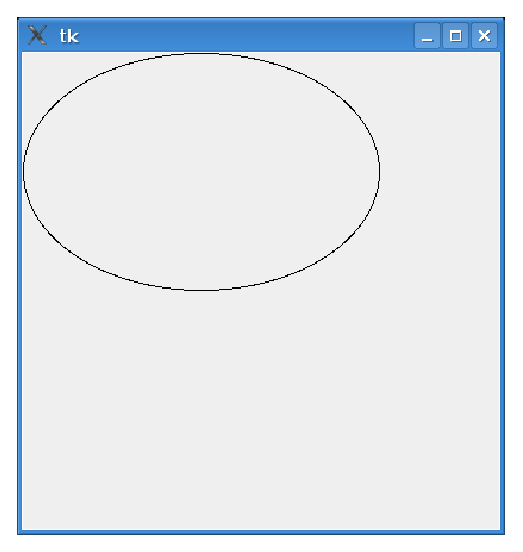
\includegraphics[width=80mm]{eps/figure38.eps}
\end{center}
\caption{O contorno da forma oval.}\label{fig38}
\end{figure}

\begin{figure}
\begin{center}
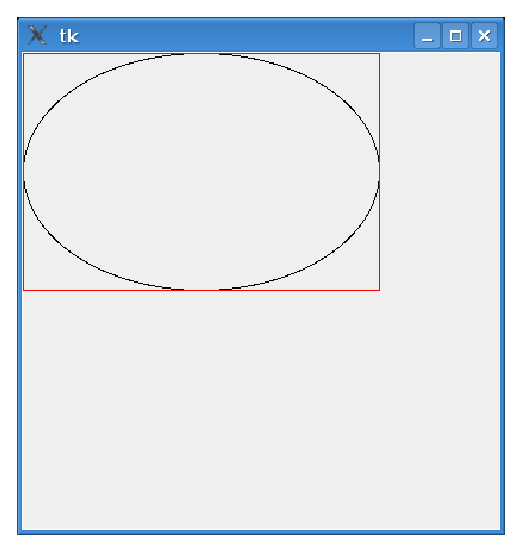
\includegraphics[width=80mm]{eps/figure39.eps}
\end{center}
\caption{O contorno da forma oval dentro de um retângulo.}\label{fig39}
\end{figure}

\noindent
Para desenhar um círculo, ao invés de uma forma oval, o retângulo imaginário deve ser um quadrado (que produz o círculo da figura~\ref{fig40}):

\begin{listing}
\begin{verbatim}
>>> tk = Tk()
>>> canvas = Canvas(tk, width=400, height=400)
>>> canvas.pack()
>>> canvas.create_oval(1, 1, 300, 300)
\end{verbatim}
\end{listing}

\begin{figure}
\begin{center}
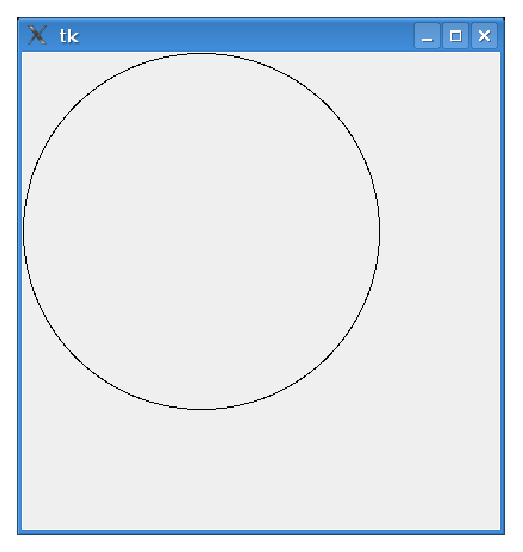
\includegraphics[width=80mm]{eps/figure40.eps}
\end{center}
\caption{Um círculo simples.}\label{fig40}
\end{figure}

\section{Desenhando Poligonos}\index{modules!tkinter!create\_polygon}

Um polígono é uma forma com 3 ou mais lados. Triângulos, quadrados, retângulos, pentágonos, hexágonos etc são todos exemplos de polígonos. Além dessas formas mais comuns, você também pode criar polígonos irregulares. Por exemplo, para desenhar um triângulo, você precisa especificar 3 pares de coordenadas para cada ponto do triângulo (criando o triângulo da figura~\ref{fig41}):

\begin{listing}
\begin{verbatim}
>>> from tkinter import *
>>> tk = Tk()
>>> canvas = Canvas(tk, width=400, height=400)
>>> canvas.pack()
>>> canvas.create_polygon(10, 10, 100, 10, 100, 50, fill="", outline="black")
\end{verbatim}
\end{listing}

\begin{figure}
\begin{center}
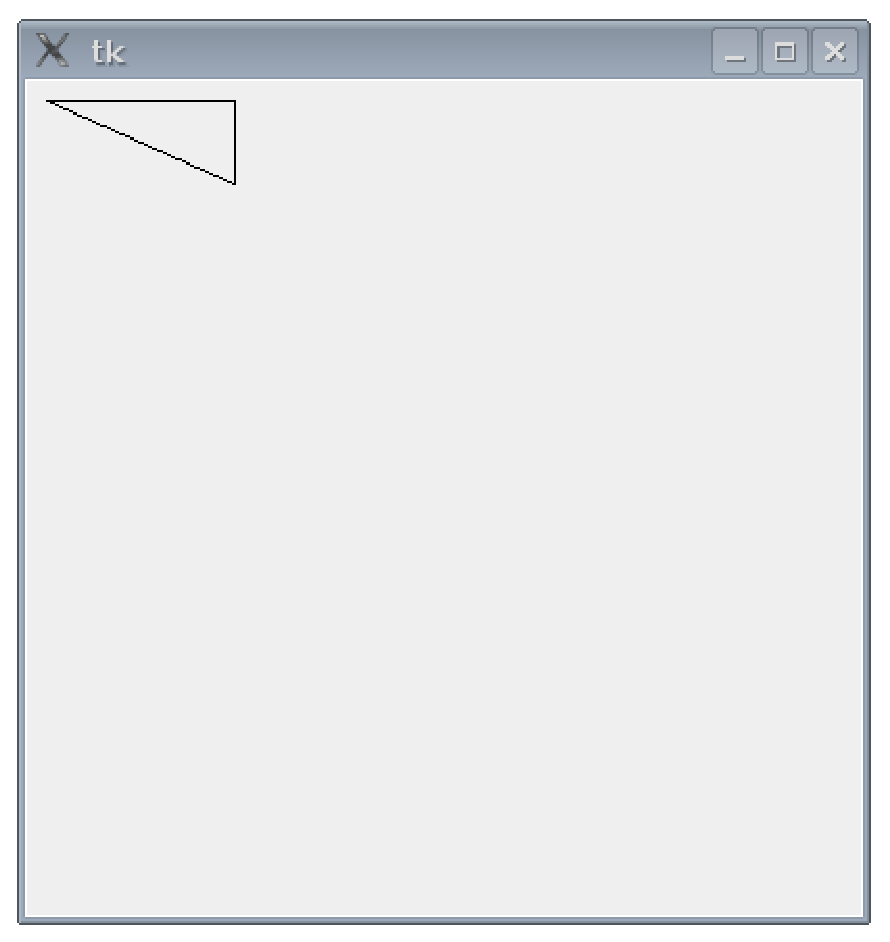
\includegraphics[width=80mm]{eps/figure41.eps}
\end{center}
\caption{Um triângulo simples.}\label{fig41}
\end{figure}

Nós podemos adicionar um polígono irregular, usando o seguinte código: A figura~\ref{fig42} exibe o triângulo e o polígono irregular.

\begin{listing}
\begin{verbatim}
>>> canvas.create_polygon(200, 10, 240, 30, 120, 100, 140, 120, fill="", outline="black")
\end{verbatim}
\end{listing}

\begin{figure}
\begin{center}
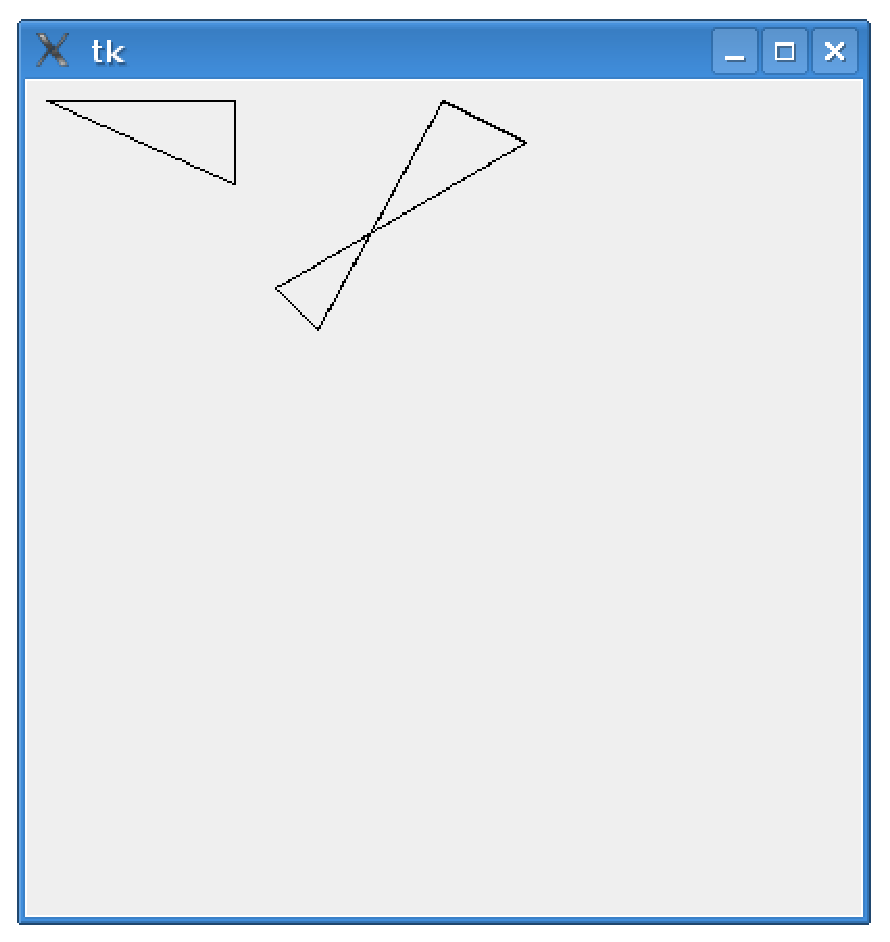
\includegraphics[width=80mm]{eps/figure42.eps}
\end{center}
\caption{Um triângulo simples e um polígono e irregular.}\label{fig42}
\end{figure}

\section{Drawing Images}

You can draw an image on a canvas using \code{tkinter} by first loading the image, then using the \code{create\_image}\index{modules!tkinter!create\_image} function on the canvas object. This sounds a bit illogical, but it works as follows:

\begin{listing}
\begin{verbatim}
1. >>> from tkinter import *
2. >>> tk = Tk()
3. >>> canvas = Canvas(tk, width=400, height=400)
4. >>> canvas.pack()
5. >>> myimage = PhotoImage(file='test.gif')
6. >>> canvas.create_image(0, 0, image=myimage, anchor=NW)
\end{verbatim}
\end{listing}

In lines 1 to 4 we set up the canvas the same as we have in previous examples. In line 5, the image is loaded into the variable \code{myimage}. It's important that the image you want to load is in a directory that's accessible to Python. This is usually the directory that the Python console is running from. You can find out the name of this directory by importing the \code{os}\index{modules!os} module and using the \code{getcwd()} function:

\begin{listing}
\begin{verbatim}
>>> import os
>>> print(os.getcwd())
\end{verbatim}
\end{listing}

\begin{WINDOWS}
This will probably print out something like `c:\\Python30'.
\end{WINDOWS}

\begin{MAC}
This will probably print out something like `/Users/yourname'$\ldots$, so if your name is Jane Matthews, \code{getcwd()} might return `/Users/janematthews'.
\end{MAC}

\begin{LINUX}
This will probably print out something like `/home/yourname'$\ldots$, so if your name is Jane Matthews, \code{getcwd()} might return `/home/jane' or `/home/janematthews', depending upon how your computer has been setup.
\end{LINUX}

Copy your image into that directory and then load it using the PhotoImage function (same as line 5). You then use the \code{create\_image} function on the canvas to display your image (line 6). If you've done all this correctly, you'll see something like figure~\ref{fig43}.

\begin{figure}
\begin{center}
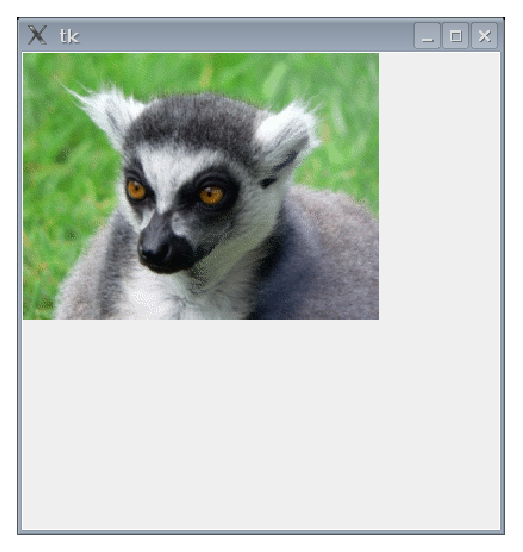
\includegraphics[width=80mm]{eps/figure43.eps}
\end{center}
\caption{A photo image.}\label{fig43}
\end{figure}

PhotoImage can load image files with the extensions .gif, .ppm and .pgm. If you want to load other types of images (there are lots of different ways you can create image files---for example, digital cameras usually store images with the extension .jpg), then you'll need to use an extension which adds that capability to Python. The Python Imaging Library (PIL)\footnote{The Python Imaging Library can be found at \href{http://www.pythonware.com/products/pil/index.htm}{http://www.pythonware.com/products/pil/index.htm}} adds the ability to load all kinds of images, as well as do things like expand and shrink, change image colours, reverse images and so on. However, installing and using the Python Imaging Library, is a bit beyond the scope of this book.

\section{Basic Animation}\index{modules!tkinter!basic animation}

So far, we've seen how to do static drawing---that's pictures that don't move. What about animation? Animation is not necessarily \code{Tk}'s strong suit, but you can do the basics. For example, we can create a filled triangle and then make it move across the screen using the following code:

\begin{listingignore}
\begin{verbatim}
1.  >>> import time
2.  >>> from tkinter import *
3.  >>> tk = Tk()
4.  >>> canvas = Canvas(tk, width=400, height=400)
5.  >>> canvas.pack()
6.  >>> canvas.create_polygon(10, 10, 10, 60, 50, 35)
7.  1
8.  >>> for x in range(0, 60):
9.  ...     canvas.move(1, 5, 0)
10. ...     tk.update()
11. ...     time.sleep(0.05)
\end{verbatim}
\end{listingignore}

The moment you press the Enter key after typing the last line, the triangle will start moving across the screen (you can see it half-way across in figure~\ref{fig44}).

\begin{figure}
\begin{center}
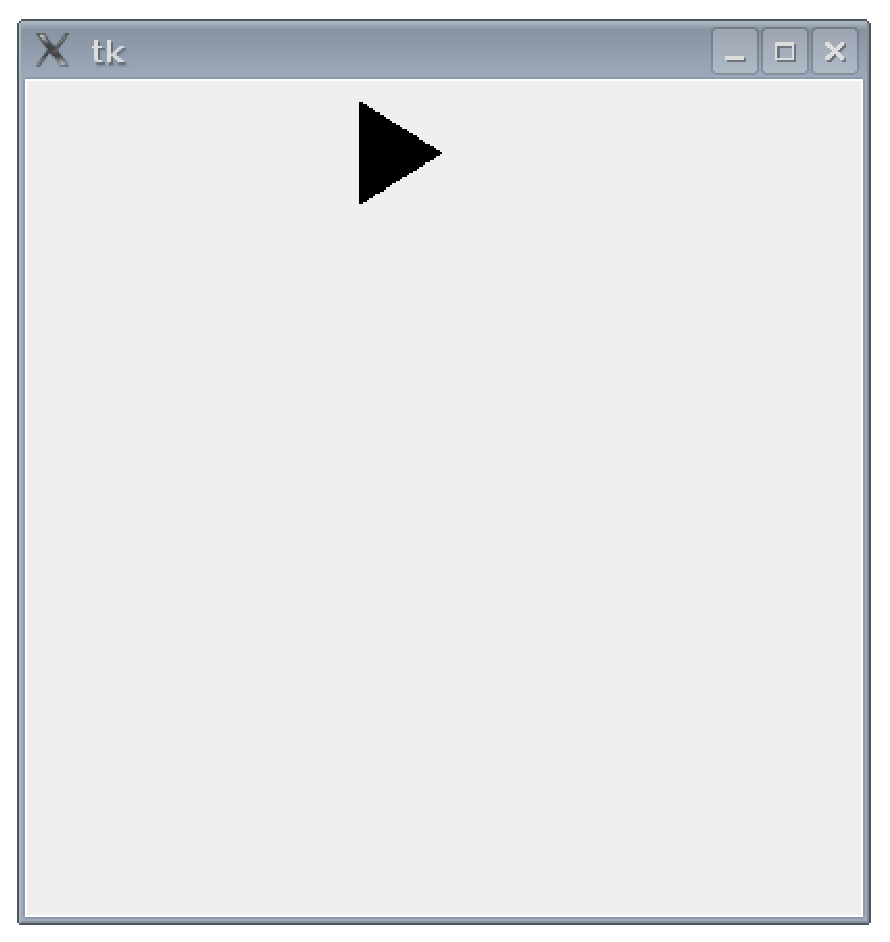
\includegraphics[width=80mm]{eps/figure44.eps}
\end{center}
\caption{The triangle moving across the screen.}\label{fig44}
\end{figure}

\par
\emph{How does it work?}
\par
Lines 1 to 5 we've seen before---it's just the basic setup to display a canvas---and in line 6, we create the triangle (using the \code{create\_polygon} function), and in line 7 you can see the identifier (the number 1) that is returned by this function. In line 8, we setup a simple for-loop to count from 0 to 59.

The block of lines (9 to 11) is the code to move the triangle. The \code{move} function on the canvas object will move any drawn object by adding values to the object's x and y coordinates. For example, in line 9 we move the object with id 1 (the identifier for the triangle) 5 pixels across and 0 pixels down. If we wanted to move the back again we might use canvas.move(1, -5, 0)\index{modules!tkinter!move}.
 
The function \code{update} on the \code{tk} object forces it to update (if we didn't use \code{update}, tkinter would wait until the loop had finished before moving the triangle, which means you wouldn't see it move). Finally line 11 tells Python to sleep for 1/20th of a second (0.05), before continuing. We can change this code, so the triangle moves diagonally down the screen, by calling \code{move(1, 5, 5)}.  First, close the canvas (by clicking on the X button on the window), then try this code:

\begin{listingignore}
\begin{verbatim}
>>> import time
>>> tk = Tk()
>>> canvas = Canvas(tk, width=400, height=400)
>>> canvas.pack()
>>> canvas.create_polygon(10, 10, 10, 60, 50, 35)
1
>>> for x in range(0, 60):
...     canvas.move(1, 5, 5)
...     tk.update()
...     time.sleep(0.05)
...
\end{verbatim}
\end{listingignore}

Figure~\ref{fig45} shows the triangle part way down the screen. Move the triangle diagonally back up the screen to its starting position, by using -5, -5:

\begin{listing}
\begin{verbatim}
>>> import time
>>> for x in range(0, 60):
...     canvas.move(1, -5, -5)
...     tk.update()
...     time.sleep(0.05)
\end{verbatim}
\end{listing}

\begin{figure}
\begin{center}
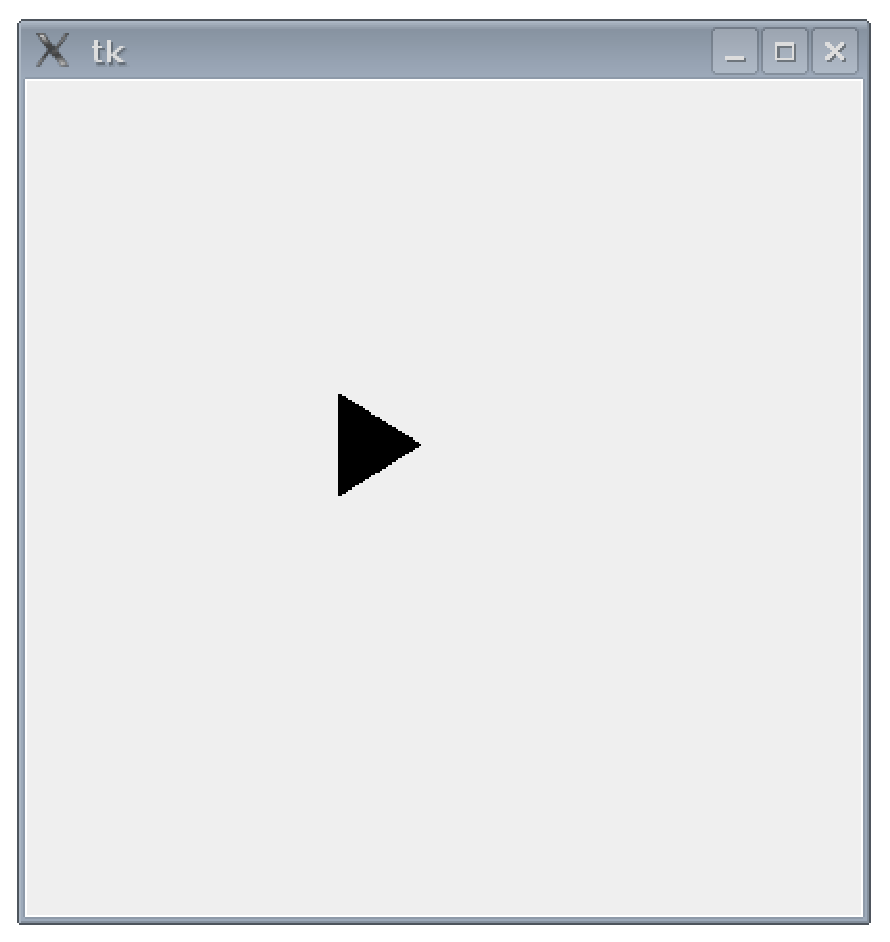
\includegraphics[width=80mm]{eps/figure45.eps}
\end{center}
\caption{The triangle moving down the screen.}\label{fig45}
\end{figure}

\section{Reacting to events$\ldots$}\index{modules!tkinter!events}

We can also make the triangle react when someone hits a key, by using what are called \emph{event bindings}.  Events are things that occur while a program is running, such as someone moving the mouse, hitting a key, or even closing a window. You can setup \code{Tk} to look out for these events, and then do something in response. To begin handling events we need to start by creating a function. Suppose we want the triangle to move when the enter key is pressed? We can define a function to move the triangle:

\begin{listing}
\begin{verbatim}
>>> def movetriangle(event):
...     canvas.move(1, 5, 0)
\end{verbatim}
\end{listing}

The function needs to have a single parameter (event), which is used by Tk to send information to the function about what has happened.  We then tell Tk that this function should be used for a particular event, using the \code{bind\_all}\index{modules!tkinter!bind\_all} function on the canvas. The full code looks like this:

\begin{listing}
\begin{verbatim}
>>> from tkinter import *
>>> tk = Tk()
>>> canvas = Canvas(tk, width=400, height=400)
>>> canvas.pack()
>>> canvas.create_polygon(10, 10, 10, 60, 50, 35)
>>> def movetriangle(event):
...     canvas.move(1, 5, 0)
...
>>> canvas.bind_all('<KeyPress-Return>', movetriangle)
\end{verbatim}
\end{listing}

The first parameter in the \code{bind\_all} function describes the event which we want Tk to look out for. In this case, it's the event \code{<KeyPress-Return>} (which is a press of the enter key).  We tell Tk that the \code{movetriangle} function should be called when this key-press event occurs.  If you run this code, click on the Tk canvas with your mouse, and then try hitting the Enter (or Return) key on your keyboard.

How about changing the direction of the triangle depending upon different key presses, such as the arrow keys? First of all we change the \code{move} triangle function to the following:

\begin{listing}
\begin{verbatim}
>>> def movetriangle(event):
...     if event.keysym == 'Up':
...         canvas.move(1, 0, -3)
...     elif event.keysym == 'Down':
...         canvas.move(1, 0, 3)
...     elif event.keysym == 'Left':
...         canvas.move(1, -3, 0)
...     else:
...         canvas.move(1, 3, 0)
\end{verbatim}
\end{listing}

The event object that is passed to \code{movetriangle}, contains a number of \emph{properties}\footnote{Properties are named values, which describe something---for example, a property of the sky is that it's blue (sometimes), a property of a car is that it has wheels. In programming terms, a property has a name and a value.}.  One of these properties is \code{keysym}, which is a string holding the value of the actual key pressed.  If \code{keysym} contains the string `Up', we call \code{canvas.move} with the parameters (1, 0, -3); if it contains down we call with the parameters (1, 0, 3), and so on.  Remember that the first parameter is the identifying number for the shape drawn on the canvas, the second parameter is the value to add to the x (horizontal) coordinate, and the last parameter is the value to add to the y (vertical) coordinate. We then tell Tk that the \code{movetriangle} function should be used to handle events from 4 different keys (up, down, left and right).  So, the code now looks like this:

\begin{listingignore}
\begin{verbatim}
>>> from tkinter import *
>>> tk = Tk()
>>> canvas = Canvas(tk, width=400, height=400)
>>> canvas.pack()
>>> canvas.create_polygon(10, 10, 10, 60, 50, 35)
1 
>>> def movetriangle(event):
...     if event.keysym == 'Up':
...         canvas.move(1, 0, -3)
...     elif event.keysym == 'Down':
...         canvas.move(1, 0, 3)
...     elif event.keysym == 'Left':
...         canvas.move(1, -3, 0)
...     else:
...         canvas.move(1, 3, 0)
... 
>>> canvas.bind_all('<KeyPress-Up>', movetriangle)
>>> canvas.bind_all('<KeyPress-Down>', movetriangle)
>>> canvas.bind_all('<KeyPress-Left>', movetriangle)
>>> canvas.bind_all('<KeyPress-Right>', movetriangle)
\end{verbatim}
\end{listingignore}

\noindent
With this example, the triangle now moves in the direction of the arrow key that you press.

\newpage
